\newpage
{\bfseries МРНТИ 52.13.17}
\hfill {\bfseries \href{https://doi.org/10.58805/kazutb.v.2.23-355}{https://doi.org/10.58805/kazutb.v.2.23-355}}

\sectionwithauthors{S.K. Moldabayev, A.A. Adamchuk, N.O. Sarybayev, A.S. Moldabayev, A.N. Nurmanova}{DEVELOPMENT AND SUBSTANTIATION OF ROCK UNLOADING DEVICE WITH
THROUGH-PASSING OF TRUCKS}

\begin{center}
{\bfseries \textsuperscript{1}S.K. Moldabayev\textsuperscript{🖂}, \textsuperscript{2}A.A. Adamchuk, \textsuperscript{1}N.O. Sarybayev, \textsuperscript{1}A.S. Moldabayev, \textsuperscript{1}A.N. Nurmanova}

\textsuperscript{1}Satbayev University, Almaty, Kazakhstan,

\textsuperscript{2}Dnipro University of Technology, Dnipro, Ukraine,

{\bfseries \textsuperscript{🖂}}Corresponding author:
s.moldabayev@satbayev.university
\end{center}

Different types of constructions of transshipment devices for combined
schemes of automobile-conveyor transport are analyzed. A device of a new
design was developed based on the identified shortcomings of known
devices. The efficiency of the rock unloading device with
through-passing trucks has been checked for the conditions of iron-ore
mines in Kazakhstan.

New device works because of rock weight force, which rotates bridges,
that cover bunker for truck to move above it. Rotating bridges makes it
possible to move rock down to bunker. After that, bridges close because
of counterweight, which is a fence at the same time.

The efficiency criteria of rock unloading device is volume reduction of
mining capital works. Parameters were considered: width of the open-cast
mine at the top and bottom, design depth of the mine, load capacity,
turning radius and width of trucks, as well as the cost of extracting 1
m\textsuperscript{3} of rock.

The dependence of reducing the costs of conducting mining capital works
in deep open-cast mines during the construction of a transshipment point
of combined automobile-conveyor transport with a through passage when
unloading trucks from their carrying capacity have been established.

{\bfseries Keywords:} combined automobile-conveyor transport,
through-passing trucks, rock unloading device, mining capital works.

\begin{center}
{\large\bfseries РАЗРАБОТКА И ОБОСНОВАНИЕ УСТРОЙСТВА РАЗГРУЗКИ СКАЛЬНОЙ ПОРОДЫ
АВТОСАМОСВАЛАМИ СО СКВОЗНЫМ ПРОЕЗДОМ}

{\bfseries \textsuperscript{1}С.K. Молдабаев\textsuperscript{🖂},
\textsuperscript{2}A.A. Aдамчук, \textsuperscript{1}Н.О. Сарыбаев,
\textsuperscript{1}A.С. Молдабаев, \textsuperscript{1}A.Н. Нурманова}

\textsuperscript{1}Сатпаев Университет, Алматы, Казахстан,

\textsuperscript{2}Национальный технический университет «Днепровская
политехника», Днепр, Украина,

e-mail: s.moldabayev@satbayev.university
\end{center}

Проанализированы различные типы конструкций перегрузочных устройств для
комбинированных схем автомобильно-конвейерного транспорта. Устройство
новой конструкции разработано с учетом выявленных недостатков известных
устройств. Работоспособность устройства разгрузки скальной породы
автосамосвалами со сквозным проездом проверена в условиях железорудных
карьеров Казахстана.

Новое устройство работает за счет силы веса горной породы, которая
вращает мосты, закрывающие бункер, над которым может передвигаться
грузовик. Вращающиеся мосты позволяют перемещать камни в бункер. После
этого мосты закрываются из-за противовеса, который одновременно является
ограждением.

Критерием эффективности устройства для разгрузки породы является
сокращение объемов горно-капитальных работ. Учитывались параметры:
ширина карьера поверху и понизу, проектная глубина котлована,
грузоподъемность, радиус поворота и ширина самосвалов, а также стоимость
добычи 1 м\textsuperscript{3} горной массы.

Установлена зависимость снижения затрат на проведение горно-капитальных
работ на глубоких карьерах при строительстве перегрузочного пункта
комбинированного автомобильно-конвейерного транспорта со сквозным
проездом при разгрузке самосвалов от их грузоподъемности.

{\bfseries Ключевые слова:} комбинированный автомобильно-конвейерный
транспорт, сквозной проезд автосамосвалов, устройство для разгрузки
породы, горно-капитальные работы\emph{.}

\begin{center}
{\large\bfseries ТОҚТАУСЫЗ ӨТЕТІН САМОСВАЛДАРМЕН ТАУ ЖЫНЫСТАРЫН ТҮСІРУГЕ АРНАЛҒАН
ҚҰРЫЛҒЫНЫ ӘЗІРЛЕУ ЖӘНЕ НЕГІЗДЕУ}

{\bfseries \textsuperscript{1}С.K. Молдабаев\textsuperscript{🖂},
\textsuperscript{2}A.A. Aдамчук, \textsuperscript{1}Н.О. Сарыбаев,
\textsuperscript{1}A.С. Молдабаев, \textsuperscript{1}A.Н. Нурманова}

\textsuperscript{1}Сәтпаев Университеті, Алматы, Қазақстан,

\textsuperscript{2}Ұлттық техникалық университет «Днепр политехникалық»,
Днепр, Украина,

e-mail: s.moldabayev@satbayev.university
\end{center}

Автомобиль-конвейер көлігінің құрама сұлбалары үшін қайта тиеу
құрылғыларының конструкцияларының әртүрлі типтері талданды. Құрылғының
жаңа дизайны белгілі құрылғылардың анықталған кемшіліктерін ескере
отырып әзірленді. Қазақстандағы темір кені карьерлері жағдайында
тоқтаусыз өтуі бар самосвалдармен тау жыныстарын түсіруге арналған
құрылғының өнімділігі сыналды.

Жаңа құрылғы жүк көлігі қозғала алатын бункерді жабатын көпірлерді
айналдыратын тау жынысының салмағының күші арқылы жұмыс істейді.
Айналмалы көпірлер тастарды бункерге жылжытуға мүмкіндік береді. Осыдан
кейін көпірлер қарсы салмаққа байланысты жабылады, бұл қоршау да болып
табылады.

Тау жыныстарын түсіруге арналған құрылғының тиімділігінің критерийі
тау-кен және құрылыс жұмыстарының көлемін азайту болып табылады. Сол
үшін келесі параметрлер ескерілді: карьердің үстіңгі және төменгі
жағындағы ені, карьердің жобалық тереңдігі, жүк көтергіштігі, бұрылу
радиусы және самосвалдардың ені, сонымен қатар, тау-кен жұмыстарының
құны 1 м\textsuperscript{3} тау-жынысы массасынан.

Автосамосвалдардан жыныстарды түсіру кезінде тоқтаусыз өтуі бар құрама
автомобиль-конвейерлік көлікті ауыстырып тиеу пунктін салу кезінде терең
карьерлерде тау-кен және құрылыс жұмыстарын жүргізуге кететін шығындарды
азайтудың олардың жүк көтергіштігіне тәуелділігі белгіленді.

{\bfseries Түйін сөздер:} құрама автомобиль-конвейерлік көлік,
автосамосвалдардың тоқтаусыз өтуі, тау жыныстарын түсіруге арналған
құрылғы, тау-кен және құрылыс жұмыстары.

\begin{multicols}{2}
{\bfseries Introduction.} In the conditions of iron ore open-cast mines,
automobile-conveyor combined transport has become widespread, the
essence of the schemes of which is that the rock is transported by truck
from the pit to the concentration horizon, on which a bunker-transloader
with a coarse crushing crusher is installed (Fig. 1) {[}1{]}. The truck
unloads the rock into the bunker, which, after crushing, falls on an
inclined conveyor installed in an underground gallery, which is then
transported to the surface.

Trucks are unloaded into the bunker as follows. When approaching the
bunker, the truck reduces its speed and begins to perform dead-end
maneuvering operations. Next, the truck reverses to the opening of the
receiving bunker, stops and starts unloading. After unloading, the truck
returns to the track and drives to be uploaded.
\end{multicols}

\begin{figure}[H]
	\centering
	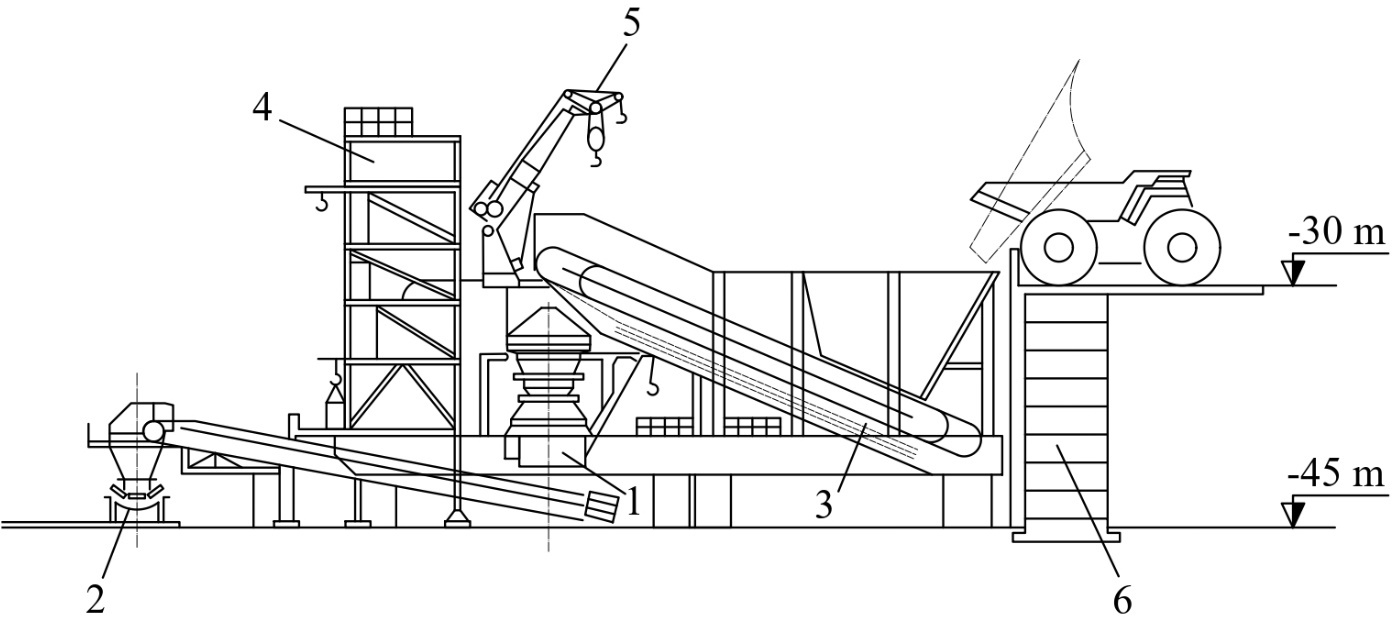
\includegraphics[width=0.7\textwidth]{assets/1350}
	\caption*{Figure 1 -- Crushing and transshipment station with dead-end unloading of trucks into a bunker:}
	\caption*{1 -- crusher; 2 -- steep belt conveyor; 3 -- plate feeder; 4 -- control panel; 5 -- lifting crane; 6 -- retaining wall {[}1{]}}
\end{figure}

\begin{multicols}{2}
To arrange a stationary transshipment point (STP), it is necessary to
have a side of the mine, placed in the final position. The STP can be
equipped with crushing and screening equipment and a bunker-accumulator.
If there is no bunker-accumulator, a warehouse of rock should be placed
near the STP with its overloading by an excavator or a wheel loader.

Trucks can be unloaded into the bunker both with a dead-end turn and
through passing. Congestion can be predicted both on the lower horizon
of the conveyor installation and on several concentration horizons. With
dead-end unloading, the crusher, screen and bunker-accumulator can be
located in the body of the ledge. Otherwise, it is necessary to provide
for the presence of a plate feeder for feeding the rock to the crusher
or overpasses for unloading trucks.

The purpose of research is to develop a new construction of rock
unloading device with through-passing of trucks and to substantiate its
effectiveness. The main tasks to achieve this purpose are: to analyze
known reloading devices with a search for their shortcomings; develop a
new design of device taking into account the identified shortcomings in
known solutions; contrast it with known designs of transfer points and
identify their shortcomings; select the criterion for the device
effectiveness; substantiate the effectiveness of the device

{\bfseries Materials and methods.} Despite the obvious advantages of
unloading trucks with through passage, some constructive solutions have
several significant disadvantages. A well-known device for unloading
trucks into a bunker (Fig. 2), which contains a rotary bridge connected
to the bunker by a hinge, a rigidly fixed counterweight on the rotary
bridge, supports, pedals for interaction with the wheels of the unloaded
truck, levers that actuate the rotary bridge, guides for the wheels of a
truck and a conveyor {[}2{]}.

The disadvantage of this device is the limited number of trucks that can
simultaneously unload into the storage bunker, which reduces the
productivity of the conveyor installation. In addition, opening the
bridge takes approximately 10--15 seconds of the truck\textquotesingle s
operating time in intensive mode due to pressing the bridge opening
lever. However, the biggest disadvantage is that there is a significant
possibility of the truck coming off the lever after pressing it and
closing the bunker cover. Re-entry of the truck in reverse for unloading
is impossible due to the presence of the lever. Thus, when using this
device, it is necessary to provide sufficiently wide platforms for the
possibility of turning around trucks. Installation of a drive for
lifting the bridge will increase the reliability of the device, but will
require additional energy {[}3--6{]}.
\end{multicols}

\begin{figure}[H]
	\centering
	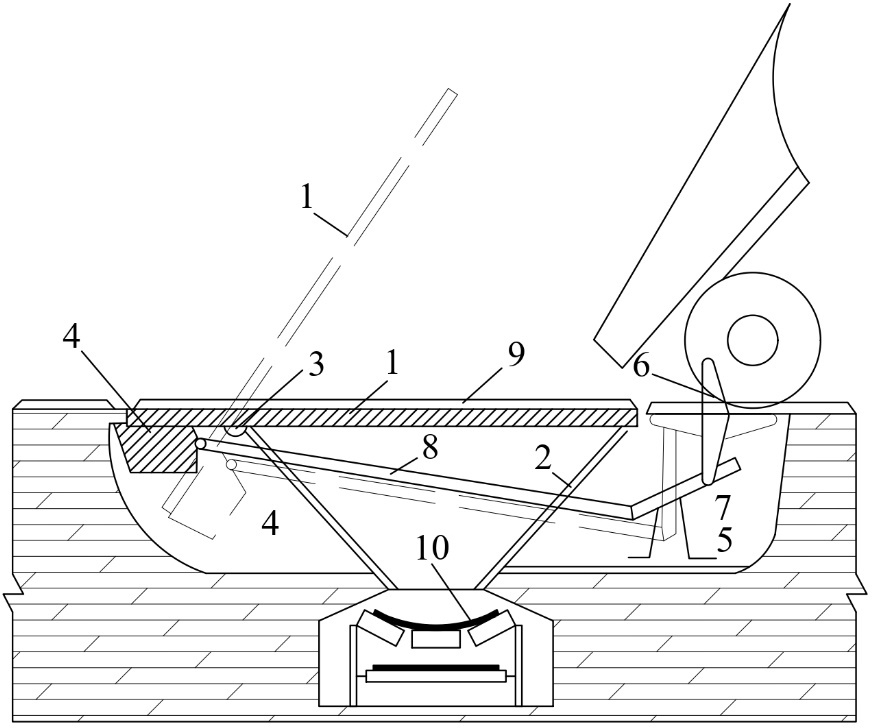
\includegraphics[width=0.5\textwidth]{assets/1351}
	\caption*{Figure 2 -- Device for unloading trucks into a bunker with hinged and lever bridge lifting:}
	\caption*{1--lifting bridge; 2 -- bunker; 3 ‒ hinge; 4 ‒ counterweight; 5 ‒ supports; 6 -- pedals; 7,8--levers;\\ 9 ‒ guides; 10 -- conveyor {[}4{]}}
\end{figure}

\begin{multicols}{2}
One of the well-known solutions is the use of a cross-moving bridge in
the design of the transshipment device (Fig. 3). Its essence is that
after passing over the bunker, the truck stops for unloading behind the
bridge. After that, the bridge on rails or rollers moves away in the
direction perpendicular to the axis of movement of the truck, then the
truck unloads the rock, after which the bridge is closed {[}7--9{]}.

This design is much simpler than the previous one, however, an
autonomous drive must be used to move the bridge, and the lid opening
time is approximately 20--30 seconds. In addition, for the construction
of a bunker of this design, an additional width of the platform for
movement of the bridge must be provided.
\end{multicols}

\begin{figure}[H]
	\centering
	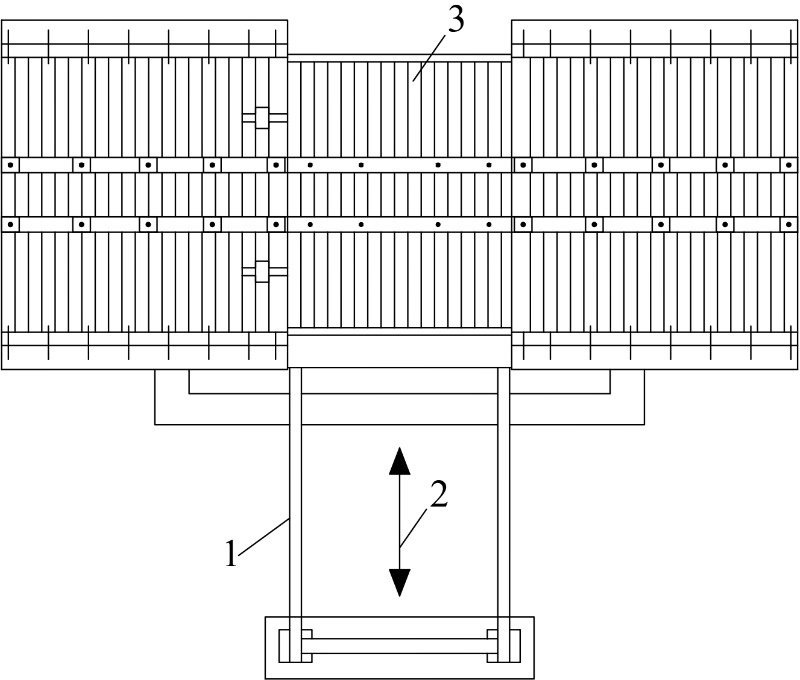
\includegraphics[width=0.5\textwidth]{assets/1352}
	\caption*{Figure 3 -- Device for unloading trucks into a bunker with a cross-moving bridge:}
	\caption*{1 -- rails; 2‒direction of movement of the cross-moving part of the bridge; 3 ‒ the middle cross-moving part of the bridge {[}9{]}}
\end{figure}

\begin{multicols}{2}
There are also known transshipment points that include a rotating
platform {[}10{]}. The principle of operation of such devices is as
follows. A truck loaded with rock drives onto the rotary platform, after
which it begins to turn around the vertical axis together with the truck
so that the latter becomes at a right angle to the axis of movement for
unloading into the bunker. After unloading the rock, the rotary platform
returns the truck to its original position, which continues moving in
the original direction.

The solution with a rotating platform allows you to significantly reduce
the width of the platform in comparison with a transshipment point with
dead-end unloading due to the reduction of the turning radius of the
truck. However, the total turning time of the platform is over 60
seconds when the truck engine is idling, and the platform has a separate
drive that uses additional energy to operate.

A number of designs of transshipment points with drive beams are known
{[}11, 12{]}. Their work consists in the fact that the loaded truck
drives over the bunker on the turning beams, unloads on them, after
which the beams rotate, due to which the rock from the surface of the
beams enters the bunker.

Among all the considered solutions, the last one has the shortest
unloading cycle time and the smallest platform width. However, the beam
drive requires additional energy expenditure for their rotation. Also,
the beams with which the truck moves must be of such a design that it
can withstand the weight of the vehicle, the impact of the unloading
rock, and at the same time correctly turn and return to the starting
position. In addition, there is a danger of failure of the stoppers,
which can cause the truck to go off the track.

In connection with the noted shortcomings of the known solutions for
unloading rocks into a bunker with through-passage of trucks, in Dnipro
University of Technology in cooperation with Satbayev University and JSC
"Sokolovsk-Sarbaisky mining and processing industrial association" (JSC
"SSMPIA") was proposed a fundamentally new solution (Fig. 4), which
differs in that after passing the truck, the rock is unloaded onto swing
bridges, which are connected hinges with beams located perpendicularly,
which move motor vehicles, while the counterweights serve as a barrier
fence, located on both sides of the beams from the outer side of the
passage and ensure the straight-line movement of trucks of the
corresponding load capacity {[}13, 14{]}.

To the reception point with the storage bunker 2, the truck 1 loaded
with rock, along the reinforced concrete beams 4, enters for unloading
between the barrier fences-counterweights 6 on the swing bridge 3 and
stops with the possibility of unloading on the nearest swing bridge 3,
which is located behind the truck 1. After unloading the rock under the
influence of its weight rotates the rotary bridges 3 in the horizontal
plane around the hinges of rotation 5 with the resolution in the open
position, and the rock falls into the storage bunker 2. Next, barrier
fences-counterweights 6 under the influence of their weight return to
their initial position and close the swing bridges 3, after which the
cycle of unloading trucks 1 to the storage bunker 2 is repeated.
\end{multicols}

\begin{figure}[H]
	\centering
	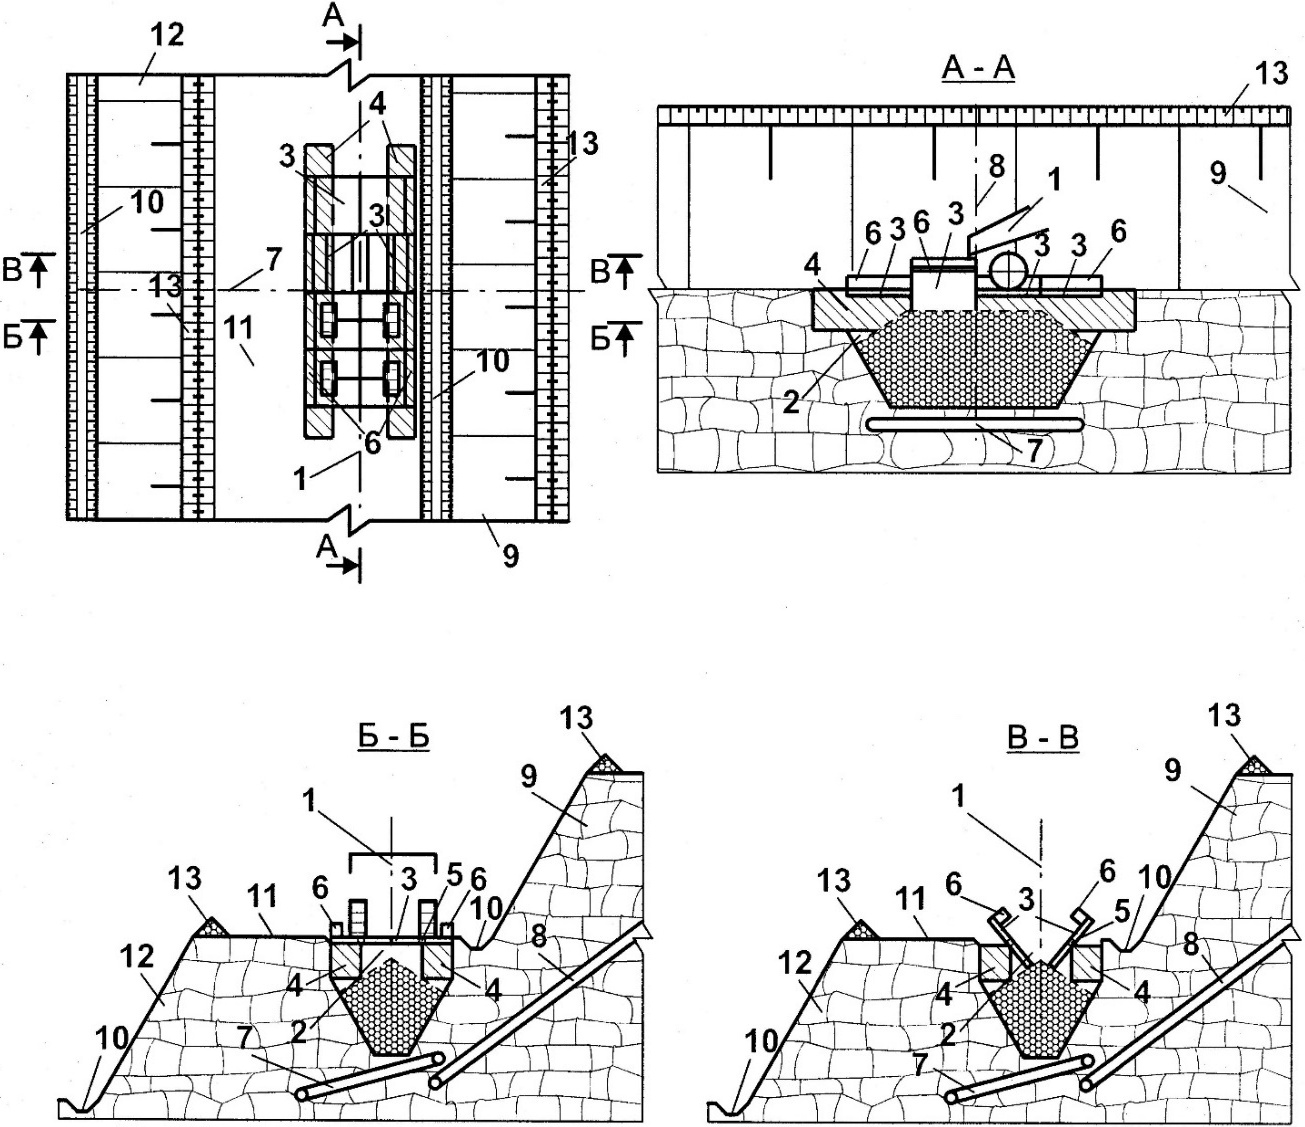
\includegraphics[width=0.8\textwidth]{assets/1353}
	\caption*{Figure 4 -- A device for unloading rocks into a bunker with through-passage of trucks {[}14{]}}
\end{figure}

\begin{multicols}{2}
After the rock reaches the bunker, it is moved through the transfer
conveyor 7 to the main conveyor 8 or the skip elevator, which transports
the rock to the surface.

To prevent groundwater from entering the storage bunker 2, a drainage
ditch 10 is constructed in the sole of the upper bench 9. To prevent
trucks 1 and other moving equipment from falling from the platform for
passing auxiliary equipment 11 to the lower bench 12, a safety rock
embankment 13 is erected on its upper edge.

The patent examiner opposed the device {[}15{]}, when the truck is
unloaded on the semi-chutes of the receiving pit, which lie on a
concrete track with a flange and are fixed to it with the possibility of
turning around the longitudinal axes. After unloading, the truck leaves
the tracks and presses the wheels on the pedal, which activates a lever
mechanism that rotates the semi-chutes, due to which the track is
cleaned.

It should be noted that lever systems cannot fully ensure the
reliability and safety of the reloading device in the conditions of
uneven cargo flows in open-pit mining operations. Large pieces of rock
can damage the elements of the half-chutes rotation mechanism. The
significant weight of heavy trucks inevitably leads to damage to the
mechanism and cannot ensure a continuous process of unloading rocks into
the bunker. In contrast to the opposite device, the rotation mechanism
of the declared one is blocked by unloading bridges, is easy to install
and operate, and the track cleaning process occurs independently of the
action of the truck, due to the action of the weight of the rock.

In addition, when unloading the rock through the opposed device, the
truck makes two stops: when unloading the rock and during track
cleaning. This leads to an increase in the unloading cycle time and, as
a result, a decrease in the throughput of the transshipment point. When
unloading through the declared device, the truck makes only one stop to
unload the rock.

The design of half-chutes in the opposite device has a complex profile,
which increases their cost and complicates the process of their
installation and operation. The claimed device provides another
implementation as unloading bridges as metal plates with counterweights
attached from the outside. Such a design can withstand dynamic loads
from the impact of large pieces of rock and ensure a continuous process
of unloading trucks regardless of the volume and composition of the
load, and the rigid fastening of the barrier fence allows, in addition
to the safety of the movement of trucks along the bridge, to turn the
bridges due to their weight in starting position.

The construction of another opposing device {[}16{]} is as follows. The
hinged-lever unloading system is attached to the framework of the
overlapping track and consists of shields pivoting relative to the
hinges, which are hingedly connected through levers and rods to the
shield channels, which cover the tracks and are hinged to them from the
inside. A fence consisting of channels and a wooden crossbar is
installed along each track from the outside.

The opposite device works as follows. A truck loaded with rock drives
along the track, stops, lifts the body and unloads. Under the influence
of the weight of the cargo, the shields turn in the vertical plane,
passing it into the bunker. After that, the overlapping shields return
to their original position under the influence of the weight of the
hinge-lever system elements.

The rotation of the unloading shields in the opposite device is brought
about, as in the claimed invention, because of the weight of the cargo.
However, the design of the claimed device differs in that it has rigidly
fixed from the outer ends of the unloading bridges of counterweights,
which are at the same time a barrier fence, and also in that the
rotation of the plates is performed due to the fact that the bridges are
movably fixed through the axis of rotation to the supports with sides of
the receiving hole. Unlike the shields, which are attached to the tracks
(beams) through hinges on their lower side, the unloading bridges in the
claimed invention are made in the form of plates, which are hinged to
the upper part of the support beam. Due to this design feature, another
system with unloading bridges can absorb more dynamically uneven loads,
including from impacts of large pieces of rock in the continuous process
of overloading the rock.

In addition, the proposed design ensures the minimum width of the
transshipment point. In the opposite device, the rotation of the shields
occurs due to the action of the hinge-lever mechanism, due to the
parameters of which the width of the transshipment point will increase.

Thus, due to the formation of a new system of connections of known
elements, namely bearing supports, on which the unloading bridges
movably fixed through the axis of rotation rest and the counterweights
rigidly attached to them at the opposite ends, which also serve as
barrier fences, a non-obvious result is achieved, which consists in the
ability to control continuous processes of unloading rock into the
bunker, regardless of their volume and composition due to the simplicity
of the design and operation of the device elements, as well as ensuring
the minimum spatial parameters of the transshipment point and the
minimum time of the unloading cycle.

{\bfseries Results and discussion.} The most important criteria of
constructing the transshipment points on open-cast mine deep horizon is
minimum amount of mining capital works, the least overburden rock
extraction. Other criteria, such as cost-effectiveness and environmental
friendliness of transport scheme, are important, but they correlate with
above-mention criteria, part of witch in overall positive effect is
about 92 \% {[}17{]}. The correlation lies in the direct relationship
between the volume of capital mining work with the cost of extracting
minerals and the amount of disturbed land. That is why substantiating
rock unloading device, taking into account the criteria of mining
capital works is sufficient.

The construction of new transshipment points, due to their significant
dimensions in plan, is connected with additional spacing of the sides of
the pit. This issue becomes especially acute in the conditions of mines
with a depth of more than 300--400 m. Thus, the minimum width of the
ledge platform on which the transshipment point is located is:
\end{multicols}

\begin{equation}
B_{1} = p + b + 2u + 2a + 3R + x + c, \, m
\end{equation}

\begin{multicols}{2}
where: \emph{p} ‒ width of the prism of possible landslide, m (3--5 m);

\emph{b} ‒ width of the safety embankment, m (1.5--3 m);

\emph{y} ‒ road shoulder width (1--1.5 m), m;

\emph{a} ‒ width of the truck, m (3.8--9.7 m);

\emph{R} ‒ turning radius of the truck, m (8.7--19.8 m);

\emph{x} ‒ safe distance between bodies of oncoming trucks, m (2--3 m);

\emph{c} ‒ safe distance between the bunker and the lower edge of the
ledge, m (5 m).

Thus, the width of the ledge platform during a dead-end turn for the
unloading of trucks is 47.2--97.8 m. However, when the trucks pass
through the bunker, the width of the ledge platform will be
significantly reduced and will be 24--48.5 m. Its value is calculated
according to the formula:

\begin{equation}
B_{2} = p + b + 2у + а + R_{\text{п}} + с, \, \text{м}.
\end{equation}

When constructing a transshipment point with through-passage of trucks
above the bunker, the volume of rocks that cannot be removed should be
determined by the formula {[}18{]}:

\begin{equation}
  \text{V}_{E}\text{=}\frac{\text{1}}{\text{6}}\text{H}^{\text{2}}\left(l + 2L \right)\left( \text{ctg}\text{α}_{1}\text{ ‒ ctg}\text{α}_{2} \right) \text{м}^{3},
\end{equation}

where: \emph{Н} -- the height of the side of the mine, m;

\emph{l}, \emph{L} -- the width of the side of the mine at the bottom
and top, m;

\emph{α\textsubscript{1}}, \emph{α\textsubscript{2}} ‒ angles of slopes
of the side of the pit when unloading trucks with a dead-end turn and
through passage over the bunker, respectively, degree.

\begin{equation}
\cot \alpha_{1} = \frac{\sum P + B_{1}}{H}, \quad \cot \alpha_{2} = \frac{\sum P + B_{2}}{H}
\end{equation}

where $\sum P$ ‒ side slope projection, m.

By substituting the expressions (4) into the formula (3), we get:

\begin{equation}
V_{\text{Е}} = \frac{1}{6} H \left( l + 2L \right) \left( B_{1} - B_{2} \right)
\end{equation}

Let\textquotesingle s consider the formulas (1) and (2):

\begin{equation}
V_{\text{Е}} = \frac{1}{6} H \left( l + 2L \right) \left( a + 2R + x \right)
\end{equation}

Thus, by constructing a transshipment point with through-passage of
trucks above the bunker at a depth of 300 m, it is possible to reduce
the volume of rock extraction by 2.7--5.7 million m\textsuperscript{3},
at a depth of 400 m by 3.5--7.5 million m\textsuperscript{3}. It is
known that extraction of 1 m3 of rock costs approx 4 USD {[}19{]}. Then,
from the point of view of extracting rocks, the savings from the
implementation of the proposed solution will amount to 10--30 million
USD {[}20{]}.

To justify the effectiveness of the proposed design, the economic effect
was calculated for the conditions of several iron ore open-cast mines in
Kazakhstan (Table 1). During the calculations, the following parameters
were taken into account: width of the pit at the top and bottom, design
depth of the pit, load capacity, turning radius and width of trucks, as
well as the cost of extracting 1 m\textsuperscript{3} of rock. Since the
load capacity, turning radius and width of trucks are related to a
specific truck model, it is proposed to take the load capacity as a
variable, as a characteristic technological parameter of a separate
truck model.

Figure 5 shows the graphs of the dependence of the total cost savings on
the development of rock for the construction of a transshipment point
with a through passage in comparison with the dead-end unloading of
trucks on their carrying capacity on the example of mines in Kazakhstan.

Graphs represent increasing polynomial functions that exist only in the
first coordinate quarter. The graphs do not cross the abscissa and
ordinate axes, and the function does not exist in the second and third
coordinate quarters, since the carrying capacity of trucks is a positive
value. The function does not exist in the fourth coordinate quarter, as
the proposed design has smaller spatial parameters and a smaller volume
of mining capital works.

The resulting dependencies allow us to assert the effectiveness of using
a transshipment point with a through passage for heavy-duty trucks at
significant depths in compressed conditions due to the reduction of the
volume of mining capital works.
\end{multicols}

\begin{table}[H]
\caption*{Table 1 -- Parameters of surface mining of iron ores in Kazakhstan}
\centering
\begin{tabular}{|p{0.3\textwidth}|p{0.1\textwidth}|p{0.1\textwidth}|p{0.1\textwidth}|p{0.1\textwidth}|p{0.1\textwidth}|}
\hline
Parameter name & Kacharsky mine & Sarbaysky mine & South Sarbai mine & Sokolovsky mine & Kurzhunkul mine \\ \hline
Mark of the mine bottom, m & -570 & -480 & -340 & -380 & -215 \\ \hline
Mine depth Нd, m & 764 & 680 & 530 & 570 & 405 \\ \hline
Geological reserves of ore Vm.g, mln t & 803,4 & 87,6 & 146,4 & 66,7 & 73 \\ \hline
\begin{tabular}[c]{@{}l@{}}Iron content in ore:\\   in deposit, \%\\   at factory, \%\end{tabular} & \begin{tabular}[c]{@{}l@{}}39,13\\   38,18\end{tabular} & \begin{tabular}[c]{@{}l@{}}38,96\\   35,5\end{tabular} & \begin{tabular}[c]{@{}l@{}}42,12\\   37,69\end{tabular} & \begin{tabular}[c]{@{}l@{}}34,8\\   28,06\end{tabular} & \begin{tabular}[c]{@{}l@{}}44,52\\   35,96\end{tabular} \\ \hline
Exploitable ore reserves Vm, mln t & 824,1 & 91,7 & 164,8 & 69,4 & 95,4 \\ \hline
The volume of overburden in mine (incl. rocks) Vr, mln m3 & \begin{tabular}[c]{@{}l@{}}956,3\\   (574,1)\end{tabular} & \begin{tabular}[c]{@{}l@{}}74,3\\   (62,5)\end{tabular} & \begin{tabular}[c]{@{}l@{}}504,7\\   (208,8)\end{tabular} & \begin{tabular}[c]{@{}l@{}}34,8\\   (34,8)\end{tabular} & 113,1 \\ \hline
Average stripping ratio ka, m3/t & 1,16 & 0,81 & 3,45 & 0,5 & 1,19 \\ \hline
\begin{tabular}[c]{@{}l@{}}Sizes of the mine on the surface:\\   – width В, m;\\   – length L, m\end{tabular} & \begin{tabular}[c]{@{}l@{}}2900\\   3000\end{tabular} & \begin{tabular}[c]{@{}l@{}}2500\\   3600\end{tabular} & \begin{tabular}[c]{@{}l@{}}1900\\   3300\end{tabular} & \begin{tabular}[c]{@{}l@{}}2000\\   3400\end{tabular} & \begin{tabular}[c]{@{}l@{}}1500\\   1500\end{tabular} \\ \hline
\begin{tabular}[c]{@{}l@{}}Sizes of the mine on the bottom:\\   – width bd, m;\\   – length ld, m\end{tabular} & \begin{tabular}[c]{@{}l@{}}175\\   430\end{tabular} & \begin{tabular}[c]{@{}l@{}}80\\   1000\end{tabular} & \begin{tabular}[c]{@{}l@{}}100\\   175\end{tabular} & \begin{tabular}[c]{@{}l@{}}70\\   200\end{tabular} & \begin{tabular}[c]{@{}l@{}}150\\   200\end{tabular} \\ \hline
\end{tabular}
\end{table}

\begin{figure}[H]
	\centering
	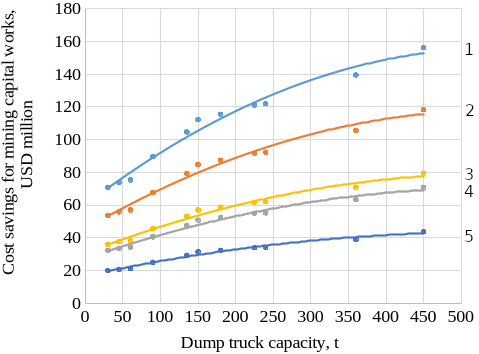
\includegraphics[width=0.6\textwidth]{assets/1363}
	\caption*{Figure 5 -- Graphs of the dependence of the total cost savings on the extraction of overburden rocks on the loading capacity of trucks when constructing a transshipment point with a through passage compared to the dead-end unloading of trucks on the example of mines in Kazakhstan:}
	\caption*{1 ‒ Kacharsky mine; 2 ‒ Sarbaysky mine; 3 ‒ Sokolovsky mine; 4 ‒ South Sarbai mine; 5 ‒ Kurzhunkul mine}
\end{figure}

\begin{multicols}{2}
{\bfseries Conclusions.} The use of a new design of the transshipment point
with the possibility of through-passage of trucks when unloading them
into the receiving bunker of the conveyor elevator is substantiated,
which allows to reduce the costs of mining and capital works.

The obtained dependences of the reduction of costs for mining and
capital works for deep open-cast mines of Kazakhstan during the
construction of a transshipment point of the combined
automobile-conveyor transport of the proposed design on the load
capacity of trucks, which allow us to assert the effectiveness of the
use of a transshipment point with through-passing of heavy trucks during
their unloading at the expense of reduction of the volume of mining and
capital works.

Currently, the degree of readiness of the developed device is a working
drawing.

\emph{{\bfseries Financing:} The article was prepared under the Grant
funding project of the Ministry of Science and Higher Education of the
Republic of Kazakhstan No. AR14869083.}
\end{multicols}

\begin{center}
{\bfseries References}
\end{center}

\begin{noparindent}
1. Dryzhenko A. Y. Vidkryti hirnychi roboty: pidruchnyk // Natsionalnyi
hirnychyi universytet.

-2014. -- 590 s. {[}in Ukraine{]}

2. Pat. 880931 Ustroistvo dlya razgruzki avtosamosvalov v bunker/ Pavlov
A.Y., Rogach M.S., Klubnichkin Y.K., Ivanova Y.Y., Propletin A.P. -№
2879141/27-11; zayavl. 30.01.80; opubl. 15.11.81, Byul. № 42. {[}in
Russian{]}

3. Pat. 713801 Ustroistvo dlya razgruzki avtosamosvalov nad bunkerom /
Markov N. G., Smetanin V. G., Istomin L. V., Dereshevatii O. Y. -№
2572759/27-11; zayavl. 10.01.78; opubl. 05.02.80, Byul. № 5. {[}in
Russian{]}

4. Pat. 135021, Ustroistvo dlya razgruzki samosvalov v bunker / Paskhin
B. M., Markozyan P. D. -№653221/27; zayavl. 04.02.1960; opubl. 1961,
Byul. № 1. {[}in Russian{]}

5. Pat. 988726, Ustroistvo dlya razgruzki avtosamosvalov v bunker /
Anikin N.N., Kuprii V.T., Chaikovskii A.I. -№3329001/27-11; zayavl.
10.08.81; opubl. 15.01.83, Byul. № 2 . {[}in Russian{]}

6. Pat. 718346 Ustroistvo dlya razgruzki avtosamosvalov v bunker /
Tartakovskii B.N., Krimskii V.I.,

Andryushchenko A.V., Lashko V.T.,
Anikin N.N. zayavl. 31.07.78; opubl. 28.02.80, Byul. № 8. {[}in
Russian{]}

7. Pat. 132123 Ustroistvo dlya razgruzki samosvalov v bunker / Paskhin
B.M., Popov A.N. -648928/27; zayavl. 29.12.1959; opubl. 1960, Byul. №
18. {[}in Russian{]}

8. Pat. 933589 Ustroistvo dlya razgruzki avtosamosvalov v bunker /
Anikin N. N., Chaikovskii A. I., Parshkin E. M. -№3008935/27-11; zayavl.
26.11.80; opubl. 10.06.82, Byul. № 21. . {[}in Russian{]}

9. Pat. 1090649 Ustroistvo dlya razgruzki samosvalov / Drizhenko A.Yu.,
Shmitko A.I., Simonenko V.I., Kritov A.Y., Birin I.S.;
zayavitel\textquotesingle{} Gosudarstvennyi institut «Yuzhgiproruda».
-№3541875/27-11; zayavl. 12.01.83; opubl. 07.05.84, Byul. №17. {[}in
Russian{]}

10. Pat. No. 1057393 Ustroistvo dlya razgruzki avtosamosvalov / Makashov
V.N., Korbinskii G.M., Drizhenko A.Y., Grinberg E.M. -№3496130/27-11;
zayavl. 27.09.82; opubl. 30.11.83, Byul. № 5.

11. Pat. 606796 Most dlya nadbunkernoi razgruzki avtosamosvalov /
Menshikov B.A., Sisin A.G. -№2363682/22-11; zayavl. 24.05.76; opubl.
15.05.78, Byul. №18. {[}in Russian{]}

12. Pat. 800077, Ustroistvo dlya nadbunkernoi razgruzki avtosamosvalov /
Budanov V.Y., Koryakin A.I., Lokhanov B.N. -№2777889/27-11; zayavl.
27.04.79; opubl. 30.01.81, Byul. № 4. {[}in Russian{]}

13. Pat. 34570 Ustroistvo dlya peregruzki skalnikh porod s
avtotransporta na konveiernii podemnik / Moldabayev S.K., Kuzmenko S.V.,
Kalyuzhnii Y.S., Drizhenko A.Y., Adamchuk A.A. -№ 2019/0143.1; zayavl.
21.02.2019; opubl. 11.09.2020. {[}in Russian{]}

14. Pat. 119491 Prystrii dlia rozvantazhennia porid iz avtosamoskydiv u
bunker / Dryzhenko A.Y., Adamchuk A.A., Shustov O.O., Moldabaiev S.K.,
Nikiforova N.A. 2019. {[}in Russian{]}

15. Pat. 120157 Priemnoe ustroistvo dlya uglya i drugikh sipuchikh i
kuskovikh materialov / Shvernik A. M., Shlikhter L.V., Tunkel N.R.
-№603176/27; zayavl. 30.06.1958; opubl. 05.02.80, Byul. № 10. {[}in
Russian{]}

16. Pat. 147533, Most dlya razgruzki sipuchikh materialov v bunkeri i
rudospuski / Anistratov Y.I., Rzhevskii V.V., Karetnikov V.N., Lyapin
L.A. -№732907/27; zayavl. 01.06.1961; opubl. 1962, Byul. № 10. {[}in
Russian{]}

17. Adamchuk A. A., Shustov O. O. Systemnyi pidkhid do vyboru novykh
zasobiv transportu dlia roboty na hlybokykh kar'ierakh // Zbirnyk
Naukovykh Prats Natsionalnoho Hirnychoho Universytetu. -2018. -№54. -S.
8-18. --URL: http://ir.nmu.org.ua/handle/123456789/152728 {[}in
Ukraine{]}

18. Adamchuk A. A. Issledovanie parametrov dorabotki glubokikh karerov
otkritim sposobom. //Zbirnyk Naukovykh Prats Natsionalnoho Hirnychoho
Universytetu (Collection of Scientific Papers of The National Technical
University). -2017. - № 50. - S. 10--17. {[}in Ukraine{]}

19. Babets Y. K., Melnykova I. Y., Hrebeniuk S. Y., Lobov S. P.
Doslidzhennia tekhniko-ekonomichnykh pokaznykiv hirnychodobuvnykh
pidpryiemstv Ukrainy ta efektyvnosti yikh roboty v umovakh zminnoi
kon'iunktury svitovoho rynku zalizorudnoi syrovyny: monograph / vyd.
R.A. Kozlov //Study of technical and economic indicators of mining
enterprises of Ukraine and their efficiency in the conditions of
changing the global market of iron ore raw materials): monohrafiia.
-2015. -391 s. {[}in Ukraine{]}

20. Adamchuk A. A. Obgruntuvannia skhemy avtomobilno-konveiernoho
transportu iz naskriznym proizdom avtosamoskydiv pry rozvantazhenni.
(Justification of the auto-conveyor transport scheme with truck through
passing while unloading) // Fiziko-Tekhnicheskie Problemi Gornogo
Proizvodstva: Sb. Nauchn. Tr. (Physical-technical problems of mining:
Collection of scientific works) -- 2021.- №~23.- S.200-215. DOI
10.37101/ftpgp23.01.013 {[}in Ukraine{]}
\end{noparindent}

\emph{{\bfseries Information about authors}}

\begin{noparindent}
Moldabayev S.- Doctor of Technical sciences, Professor, Satbayev
University, Almaty, Kazakhstan, e-mail:

s.moldabayev@satbayev.university;

Adamchuk A. -- Candidate of Engineering Sciences, Dnipro University of
Technology, Dnipro, Ukraine, e-mail: Adamchuk.A.A@nmu.one;

Sarybayev N. -- PhD, Satbayev University, Almaty, Kazakhstan, e-mail:
n.sarybayev@satbayev.university;

Moldabayev A.- Master's degree student, Satbayev University, Almaty,
Kazakhstan, e-mail:

asangiz.moldabaev@stud.satbayev.university;

Nurmanova A. -- PhD student, Satbayev University, Almaty, Kazakhstan,
e-mail: a.nurmanova@satbayev.university
\end{noparindent}

\emph{{\bfseries Сведения об авторах}}

\begin{noparindent}
Молдабаев С. -- доктор технических наук, профессор, Сатпаев университет,
Алматы, Казахстан, e-mail: s.moldabayev@satbayev.university;

Адамчук А. -- кандидат технических наук, Национальный технический
университет «Днепровская политехника», Днепр, Украина, e-mail:
Adamchuk.A.A@nmu.one;

Сарыбаев Н. -- PhD, Сатпаев университет, e-mail:
n.sarybayev@satbayev.university;

Молдабаев А.-студент магистратуры, Сатпаев университет, Алматы,
Казахстан, e-mail:

asangiz.moldabaev@stud.satbayev.university;

Нурманова А.- студент PhD, Сатпаев университет, Алматы, Казахстан,
e-mail:

a.nurmanova@satbayev.university/
\end{noparindent}
